% SPDX-License-Identifier: CC-BY-SA-4.0
% Author: Matthieu Perrin
% Part: 
% Section: 
% Sub-section: 
% Frame: 

\begingroup

\begin{frame}{Analyse contextuelle}

  \begin{tikzpicture}

  \draw (10.5,7.5) node{\begin{minipage}{\textwidth}
      \begin{block}{Les grammaires algébriques ne suffisent pas toujours}
  \end{block}\end{minipage}};

      \draw[latex-latex, alert] (6.5,5.3) to[out=20,in=160] (9.4,5.3);
      \draw[latex-latex, structure] (9,4.7) to[out=-20,in=-160] (10.5,4.7);

    \draw (8.7,5) node{\og \alert{Le chat} a mangé \structure{la souris}. \alert{Il} l'a \structure{appréciée}. \fg};

  \draw (14,5) node{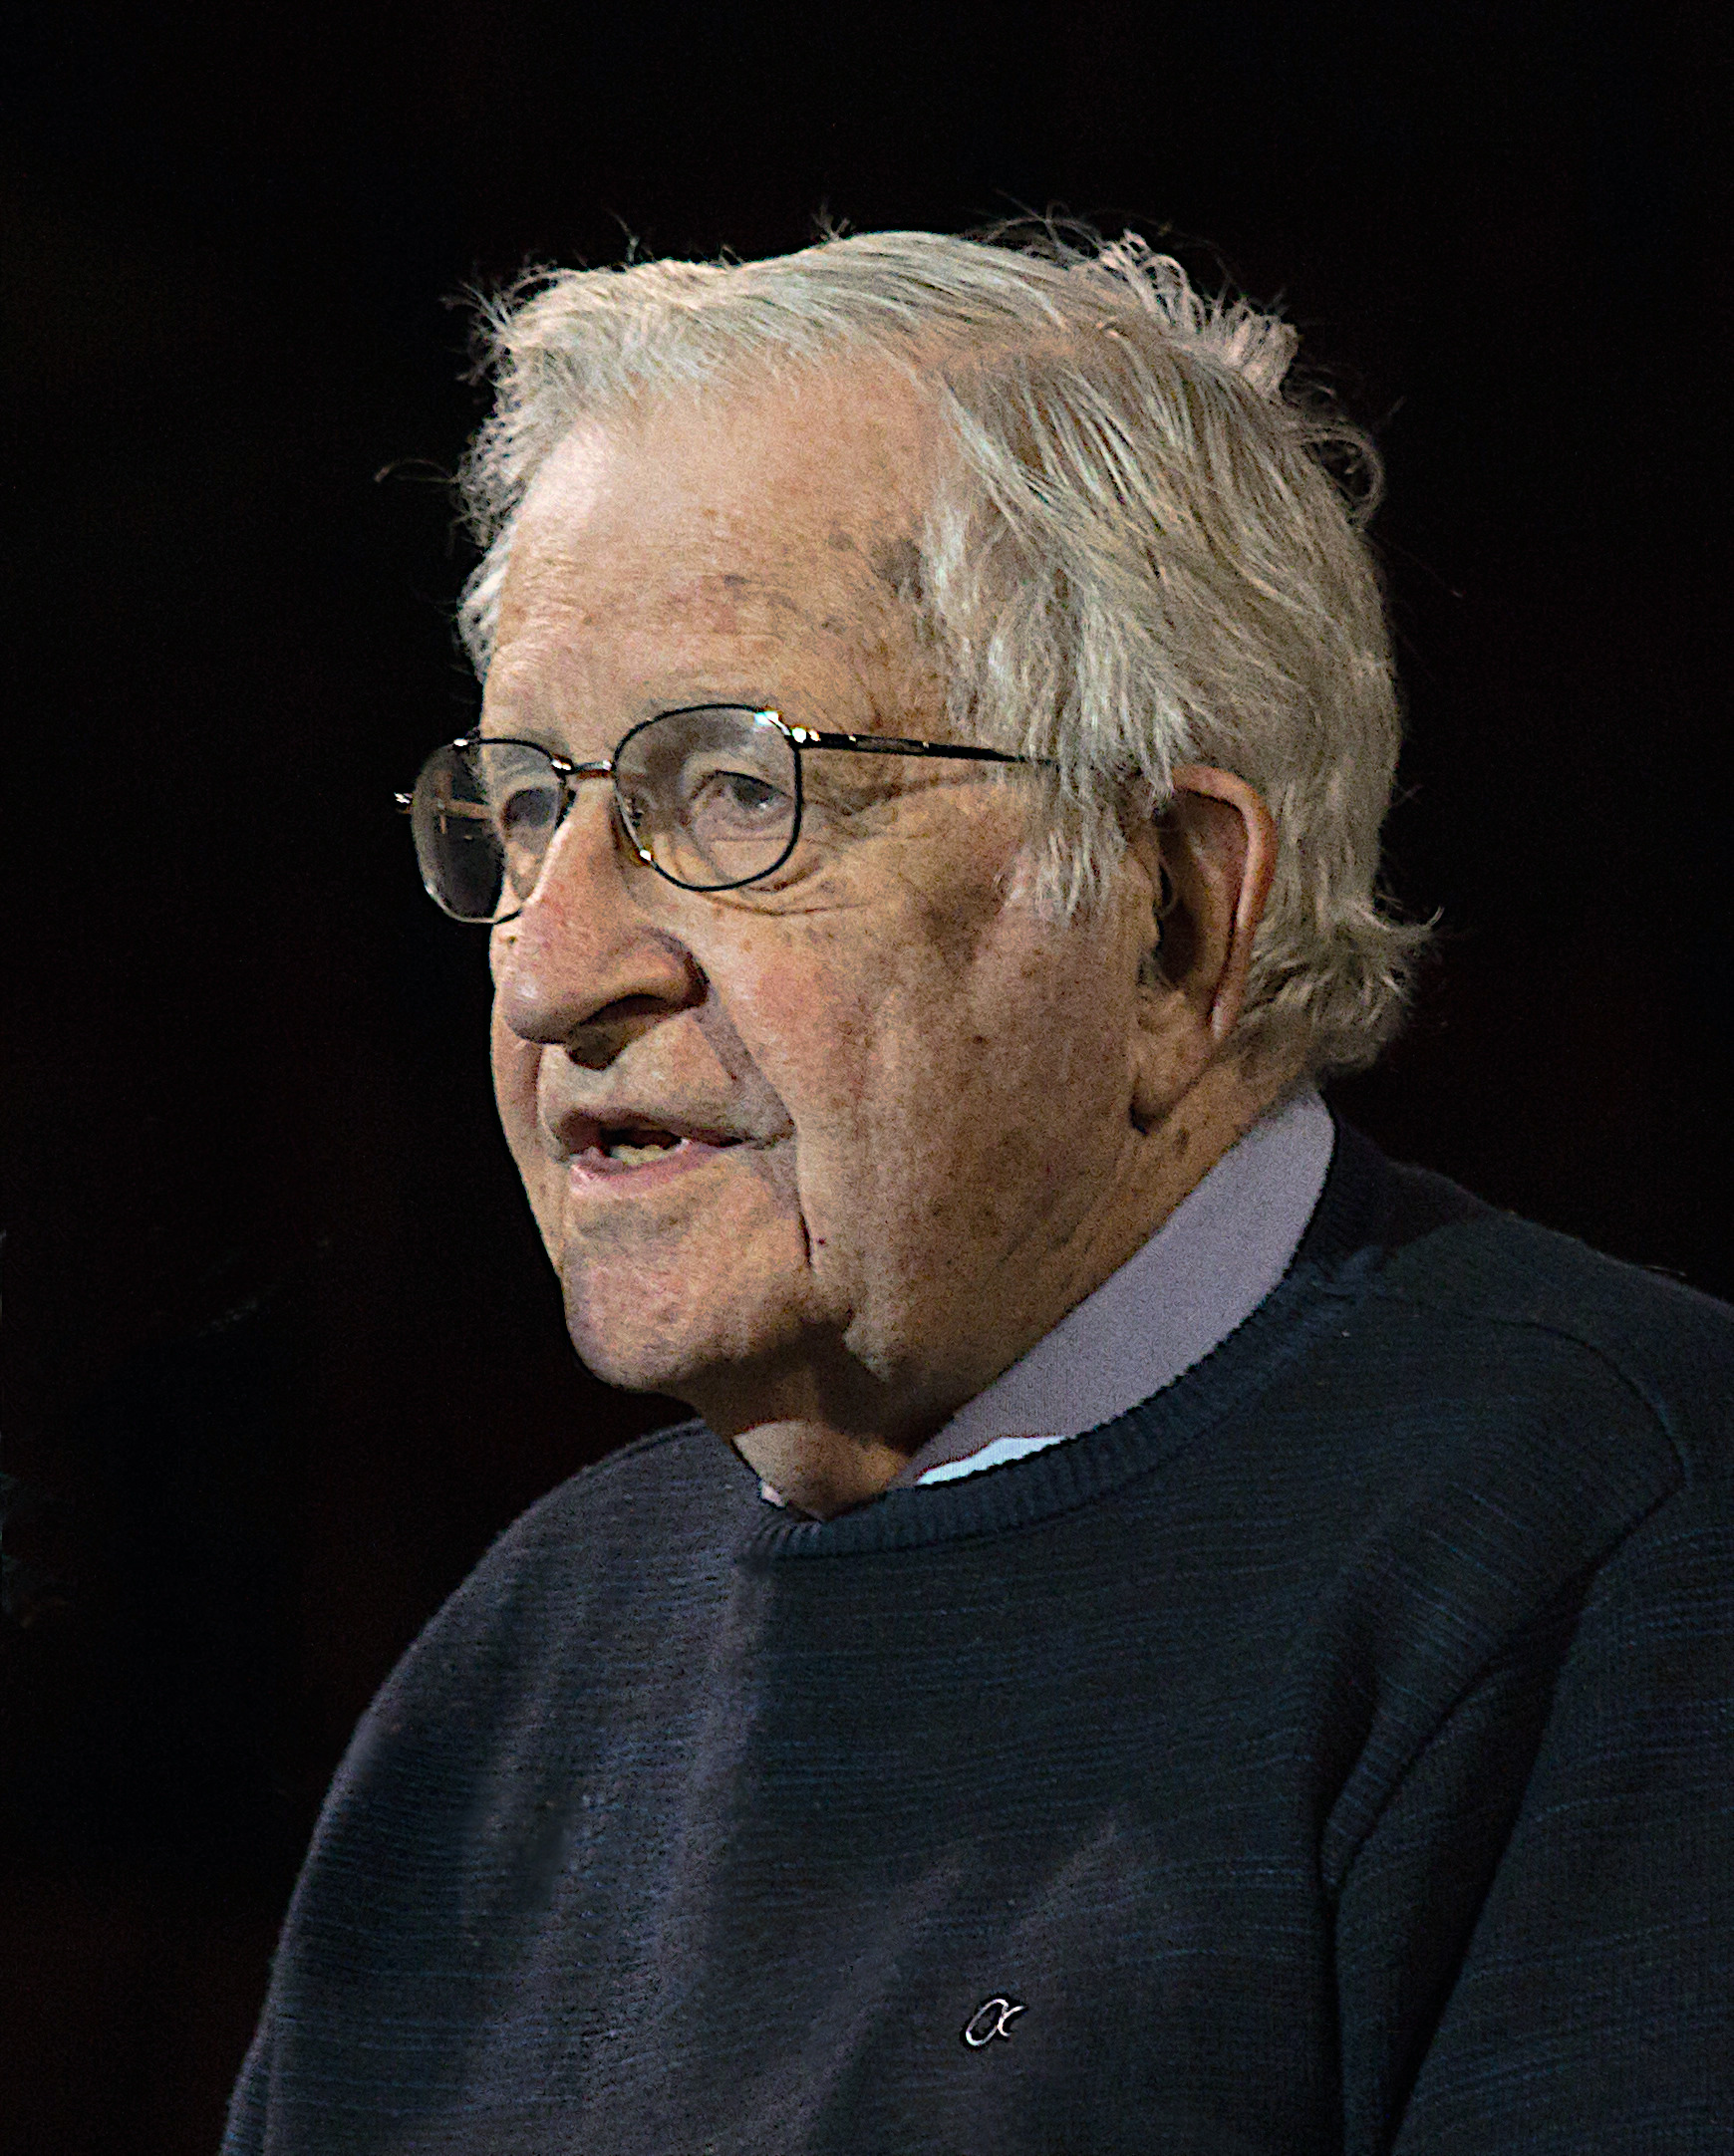
\includegraphics[width=3cm]{img/Chomsky}};
  \draw (14,2.8) node{Noam Chomsky};

  
  \draw (10.5,1.5) node{\begin{minipage}{\textwidth}
      \begin{block}{Phase d'analyse contextuelle dans la compilation}
        \begin{itemize}
        \item Vérification de la portée des variables
        \item Vérification des types
        \end{itemize}
  \end{block}\end{minipage}};

  
  \end{tikzpicture}
  
\end{frame}

\endgroup
